\documentclass[a4paper,12pt]{report}

\usepackage{cmap}
\usepackage[T2A]{fontenc}
\usepackage[utf8]{inputenc}
\usepackage[russian]{babel}
\usepackage{amsmath,amsfonts,amssymb}
\usepackage{graphicx}
\usepackage{sidecap}
\usepackage{wrapfig}
% \usepackage{pgfplots} 
% \pgfplotsset{compat = 1.18,width = 15cm}

\begin{document} 

\begin{titlepage} 

\begin{center} 

\large Федеральное государственное автономное образовательное учреждение высшего образования «Санкт-Петербургский государственный электротехнический университет «ЛЭТИ» им. В.И. Ульянова (Ленина)»
	
кафедра физики\\[5cm] 


\huge ОТЧЕТ\\ по лабораторной работе № 3\\[0.5cm] 
\large <<Исследование динамики колебательного и вращательного движения>>\\[3.7cm]

\begin{minipage}{1\textwidth} 
    \begin{flushleft} 
        \emph{Автор:} Стукен В.А.\\
        \emph{Группа:} 2307\\
        \emph{Факультет:} ФКТИ\\
        \emph{Преподаватель:} Харитонский П.В. 
    \end{flushleft} 
\end{minipage} 

\vfill 

Санкт-Петербург, 2022\\
{\large \LaTeX} 

\end{center} 

\thispagestyle{empty} 
\end{titlepage} 

\section*{Работа №3 "Исследование динамики колебательного и вращательного движения"}

\begin{wrapfigure}{r}{0.2\textwidth}
    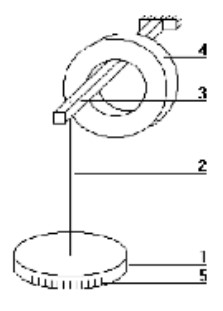
\includegraphics[width=0.2\textwidth]{ustanovka.jpg}
    \label{ris:image}
\end{wrapfigure}

\par
\textit{Цель работы:} Исследование динамики колебательного движения на примере крутильного маятника, определение момента инерции маятника, модуля сдвига материала его подвеса и характеристик колебательной системы с затуханием (логарифмического декремента затухания и добротности колебательной системы).
\textit{Приборы и принадлежности: } физический маятник;
секундомер; масштабная линейка, чертежный треугольник.

Применяемый в работе крутильный маятник представляет собой диск 1, закреплен- ный на упругой стальной проволоке 2, свободный конец которой зажат в неподвижном кронштейне 3. На кронштейне расположено кольцо 4, масса ко- торого известна. Кольцо 4 можно положить сверху на диск 1, изменив тем самым момент инерции ма- ятника. Для отсчета значений угла 
поворота маятника служит градуированная шкала 5, помещенная на панели прибора снизу от диска 1.

\section*{Исследуемые закономерности}

\par

\subsection*{Момент инерции крутильного маятника}
\par
Момент инерции (аналог инертной массы тела при его поступательном движении) - 
физическая величина, характеризующая инертные свойства твердого тела при его вращении. 
\par
Если твердое тело вращается вокруг неподвижной оси, то момент инерции относительно этой оси вычисляется как сумма произведений элементарных масс $\Delta m_i$, составляющих тело, на квадраты их расстояний $r_i$ до оси вращения. В случае сплошного тела сумма в определении момента инерции переходит в интеграл .
\par
Крутильный маятник совершает вращательное колебательное движение вокруг оси, совпадающей с направлением стальной проволоки. Используя основное уравнение динамики вращательного движения, можно определить момент инерции маятника, а также физические величины, описывающием вращательное движение. 

\newpage
\subsection*{Уравнение движения крутильного маятника}

\begin{wrapfigure}{r}{0.4\textwidth}
    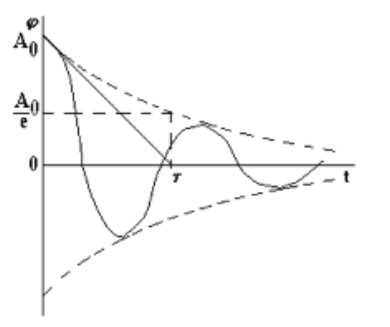
\includegraphics[width=0.3\textwidth]{graph.jpg}
    \label{ris:image}
\end{wrapfigure}

При повороте тела, закрепленного на упругом подвесе, в результате деформации сдвига возникает вращающий момент упругих сил. 
Трение в подвесе создает тормозящий момент, пропорциональный скорости движения маятника.
Исследуемый в работе крутильный маятник представляет собой сложную систему (диск с различными креплениями, прикрепленный к проволочному подвесу) с неизвестным моментом инерции $I_d$, 
который представляет собой постоянную часть исследуемой системы. Если на диск маятника положить тело с известным моментом инерции - кольцо с моментом инерции $I_k$ , то момент инерции маятника станет равным $I_d+I_k$ . 

\subsection*{Крутильный маятник как диссипативная система}

Полная энергия колебаний маятника убывает со временем. 
Убывание энергии происходит за счет совершения работы против сил трения. 
Энергия при этом превращается в тепло. 
Помимо коэффициента затухания $\beta$ (или времени затухания $\tau$) и мощности потерь $P_d$ колебательная диссипативная система характеризуется также добротностью $Q$, 
позволяющей судить о способности системы сохранять энергию. 
Добротность численно равна числу колебаний за время $t = \tau\pi$. 
За это время амплитуда колебаний уменьшается в $e^{\pi} \approx 23$ раза, 
а энергия колебаний в $e^{2\pi} \approx 535$ раз, иными словами за это время колебания практически затухают. 
Часто также используется параметр $N_e = \frac{\tau}{T}$ - число колебаний, за которое амплитуда колебаний уменьшается в $e$ раз. 

\newpage
\subsection*{Определение модуля сдвига}

\begin{wrapfigure}{r}{0.3\textwidth}
    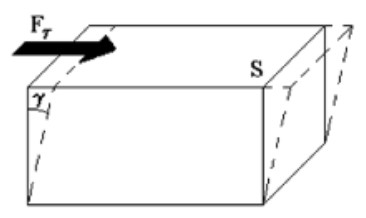
\includegraphics[width=0.3\textwidth]{sdvig.jpg}
    \label{ris:image2}
\end{wrapfigure}

Методом крутильных колебаний пользуются для косвенного измерения модуля сдвига $G$ материала подвеса. 
Модуль сдвига характеризует упругие свойства материала и в случае малых деформаций равен силе, действующей на единицу площади $S$ при единичном угле сдвига $\gamma$ касательно сдвигу слоев вещества в месте определения модуля $G$.
Модуль сдвига $G$ связан с модулем Юнга, характеризующим сопротивление материала сжатию или растяжению. Коэффициент Пуассона - отношение поперечное и продольной относительной деформации образца материала и для металлов близок к 0.3. 

\newpage

\section*{Протокол измерений}

\begin{flushleft}
    
\resizebox{16cm}{!}{ 
    \begin{tabular}{|l|l|l|l|l|l|l|l|}
        \hline
           $l$ & $d$ & $D_{ex}$ & $D_{in}$ & $D_0$ & $h_0$ & $m$ & $\rho$\\
        \hline
               &     &          &         &     &        &       & \\ 
        \hline
    \end{tabular}
}
\end{flushleft}

\resizebox{10cm}{!}{
    \begin{tabular}{|l|l|l|l|l|}
        \hline
             № & t_d & t_{0d} & $t_k$ &  $t_{0k}$ \\
        \hline
        1  &   &   &   &   \\ 
        \hline
        2  &   &   &   &   \\
        \hline
        3  &   &   &   &   \\
        \hline
        4  &   &   &   &   \\
        \hline
        5  &   &   &   &   \\
        \hline
    \end{tabular}
}


\newpage
\section*{Ответы на вопросы}

\begin{itemize}
    \item \textbf{Вопрос №9:}
    	\textit{"Физический смысл коэффициента затухания $\beta$?"} \\
        Коэффициент затухания $\beta$ характеризует скорость затухания колебаний. $\beta = \frac{1}{\tau}$
    \item \textbf{Вопрос №40:}
        \textit{"Выведите формулу:"}
         \[ I_d = \frac{I_k}{(\frac{T_{dk}}{T_d})^2-1} \]
         \[ \omega_0 = \frac{2\pi}{T} = \sqrt{\frac{D}{I_{d}}} \]
         Отсюда:
         \[ T_d = 2\pi\sqrt{\frac{I_d}{D}} \]
         \[ T = 2\pi \sqrt{(I_d + I_k)/D} \]
         Отсюда:
         \[ I_d = \frac{I_k}{(\frac{T_{dk}}{T_d})^2-1} \]
        
\end{itemize}

\newpage

\section*{Обработка результатов измерений}

\subsection*{Найдем $t_d = \bar{t_d} \pm \Delta \bar{t_d}$}

$N=5,\ \ U_{PN}=0.64,\ \ V_{PN}=1.67,\ \ \beta_{PN}=0.51,\ \ t_{PN}=2.8$\\
Промахов нет.\\
\[\bar{t}= \frac{15.66+15.66+15.72+15.76+15.91}{5} =15.742 s\] \\
\[S_{t}=\sqrt{\frac{(\bar{t}-{t}_1)^2+(\bar{t}-{t}_2)^2+(\bar{t}-{t}_3)^2+(\bar{t}-{t}_4)^2+(\bar{t}-{t}_5)^2}{N-1}} = 0.103\]\\

\[\bar{S_{t}}=\frac{S_{t}}{\sqrt{t}}=\frac{0.103}{\sqrt{5}}=0.046\]

\[\Delta{t}_{(R)}=R\cdot B_{PN}=0.25\cdot 0.51=0.128 \, s\]
\[\Delta{t}_{(\bar{S_{t}})}=\bar{S_t}\cdot t_{PN}=0.046\cdot 2.8=0.129 \, s\]
\[\Delta{\bar{t}}=\sqrt{\Delta t^2 + \theta^2}=\sqrt{0.129^2 + 0.01^2}=0.129 \, s\]

\[{t_d}=\bar{t_d}\pm \Delta{\bar{t_d}}=15.74\pm 0.12 \, s\]

\subsection*{Найдем $t_{0d} = \bar{t_{0d}} \pm \Delta \bar{t_{0d}}$}

$N=5,\ \ U_{PN}=0.64,\ \ V_{PN}=1.67,\ \ \beta_{PN}=0.51,\ \ t_{PN}=2.8$\\
Промахов нет.\\

\[\bar{t}= \frac{18.9+18.93+19.06+20.34+20.4}{5} = 19.526 \, s\]

\[S_{t}=\sqrt{\frac{(\bar{t}-{t}_1)^2+(\bar{t}-{t}_2)^2+(\bar{t}-{t}_3)^2+(\bar{t}-{t}_4)^2+(\bar{t}-{t}_5)^2}{N-1}} = 0.773\]

\[ \bar{S_{t}}=\frac{S_{t}}{\sqrt{N}}=\frac{0.773}{\sqrt{5}}=0.346 \]

\[ \Delta{t}_{(R)}=R\cdot B_{PN}=1.5\cdot 0.51=0.765 \]
\[ \Delta{t}_{(\bar{S_{t}})}=\bar{S_t}\cdot t_{PN}=0.346\cdot 2.8=0.969 \]

\[ \Delta{\bar{t}}=\sqrt{\Delta t^2 + \theta^2}=\sqrt{0.969^2 + 0.01^2}=0.969 \, s\]

\[ {t_{0d}}=\bar{t_{0d}}\pm \Delta{\bar{t_{0d}}}=19.5\pm 0.9 \, s\]


\subsection*{Найдем $t_{k} = \bar{t_{k}} \pm \Delta \bar{t_{k}}$}

$N=5,\ \ U_{PN}=0.64,\ \ V_{PN}=1.67,\ \ \beta_{PN}=0.51,\ \ t_{PN}=2.8$\\
Промахов нет.\\

\[\bar{t}= \frac{21.71+21.81+21.84+22+22.13}{5} =21.898 \]
\[S_{t}=\sqrt{\frac{(\bar{t}-{t}_1)^2+(\bar{t}-{t}_2)^2+(\bar{t}-{t}_3)^2+(\bar{t}-{t}_4)^2+(\bar{t}-{t}_5)^2}{N-1}} = 0.166\]

\[ \bar{S_{t}}=\frac{S_{t}}{\sqrt{N}}=\frac{0.166}{\sqrt{5}}=0.074 \]

\[ \Delta{t}_{(R)}=R\cdot B_{PN}=0.42\cdot 0.51=0.214 \]
\[ \Delta{t}_{(\bar{S_{t}})}=\bar{S_t}\cdot t_{PN}=0.074\cdot 2.8=0.207 \]
\[ \Delta{\bar{t}}=\sqrt{\Delta t^2 + \theta^2}=\sqrt{0.207^2 + 0.01^2}=0.207 \]

\[ {t_k}=\bar{t_k}\pm \Delta{\bar{t_k}}=21.9\pm 0.2 \, s\]

\subsection*{Найдем $t_{0k} = \bar{t_{0k}} \pm \Delta \bar{t_{0k}}$}

$N=5,\ \ U_{PN}=0.64,\ \ V_{PN}=1.67,\ \ \beta_{PN}=0.51,\ \ t_{PN}=2.8$\\
Промахов нет.\\

\[\bar{t}= \frac{17.65+17.66+17.69+17.79+17.82}{5} =17.722 \, s\]

\[S_{t}=\sqrt{\frac{(\bar{t}-{t}_1)^2+(\bar{t}-{t}_2)^2+(\bar{t}-{t}_3)^2+(\bar{t}-{t}_4)^2+(\bar{t}-{t}_5)^2}{N-1}} = 0,078\]

\[ \bar{S_{t}}=\frac{S_{t}}{\sqrt{N}}=\frac{0.078}{\sqrt{5}}=0.035 \]

\[ \Delta{t}_{(R)}=R\cdot B_{PN}=0.17\cdot 0.51=0.087 \]

\[\Delta{t}_{(\bar{S_{t}})}=\bar{S_t}\cdot t_{PN}=0.035\cdot 2.8=0.098\]

\[ \Delta{\bar{t}}=\sqrt{\Delta t^2 + \theta^2}=\sqrt{0.098^2 + 0.01^2}=0.099 \]

\[{t_{ok}}=\bar{t_{0k}}\pm \Delta{\bar{t_{0k}}}=17.72\pm 0.09 \, s\]

\subsection*{Рассчитаем $T_d = \bar{T_d} \pm \Delta \bar{T_d}$}

\[ \bar{T_d} = \frac{\bar{t_d}}{n} = 15.742/10 = 1,57 \, s \]
\[ \Delta \bar{T_d} = \frac{\Delta \bar{t_d}}{n} = 0.129/10 = 0.013 \]
\[ T_d = \bar{T_d} \pm \Delta \bar{T_d} = 1.570 \pm 0,013 \, s \]

\subsection*{Рассчитаем $T_k = \bar{T_k} \pm \Delta \bar{T_k}$}

\[ \bar{T_k} = \frac{\bar{t_k}}{n} = 21.9/10 = 2.2 \, s \]
\[ \Delta \bar{T_d} = \frac{\Delta \bar{t_d}}{n} = 0.207/10 = 0.02 \]
\[ T_k = \bar{T_k} \pm \Delta \bar{T_k} = 2.20 \pm 0.02 \, s \]

\subsection*{Рассчитаем время затухания}

\[ \tau = \frac{t_0}{\ln2} \]
\[ \bar{t_{d}} = \frac{\bar{t_{0d}}}{\ln2} = 19.526/0.693 = 28.18 \, s \]
\[ \bar{t_{k}} = \frac{\bar{t_{0k}}}{\ln2} = 17.722/0.693 = 25.57 \, s \]

\[ \tau_d = 28.18 \pm 1.4 \, s \]
\[ \tau_k = 25.57 \pm 0.14 \, s \]

\subsection*{Найдем собственную частоту колебаний \\ маятника без кольца и с кольцом}

\[ \bar{\omega_{0d}} = \frac{2\pi}{\bar{T_d}} = 4 \, s^{-1} \]
\[ \bar{\omega_{0k}} = \frac{2\pi}{\bar{T_k}} = 2.85 \, s^{-1} \]

\[ \Delta \bar{\omega_{0d}} = 0.033 \, s^{-1} \]
\[ \Delta \bar{\omega_{0k}} =  0.026 \, s^{-1}\]

\[ \omega_{0d} = 4.00 \pm 0.03 \, s^{-1} \]
\[ \omega_{0k} = 2.85 \pm 0.03 \, s^{-1} \]

\subsection*{Рассчитаем момент инерции кольца}

\[ I_k = \frac{m}{8}\biggl( D_{ex}^2 + D_{in}^2\biggr) = \frac{1.832}{8} \cdot (0.247^2 + 0.0585^2) = 0.015 \, kg\cdot m^2 \]

\subsection*{Рассчитаем момент инерции диска}

\[ I_d = \bar{I_d} \pm \Delta \bar{I_d} \]

\[ \bar{I_d} = \frac{I_k\bar{\omega_{0k}^2}}{\bar{\omega_{0d}^2}-\bar{\omega_{0k}^2}} = 0.015\]
Прологарифмировав данное выражение получим:
\[ \ln I_k + 2\ln \omega_{0k} = \ln I_d \cdot (\ln (\omega_{0d} + \omega_{0k} ) + \ln (\omega_{0d} - \omega_{0k})) \]

\[ \Delta \bar{I_d} = \sqrt{\biggl(\frac{dI_d}{d\omega_{0d}}\bigg \vert_{\bar{\omega_{0d}},\bar{\omega_{0k}}}\cdot \Delta \bar{\omega_{0d}}\biggr)^2 + \biggl(\frac{dI_d}{d\omega_{ok}}\bigg \vert_{\bar{\omega_{0d}},\bar{\omega_{0k}}}\cdot \Delta \bar{\omega_{0k}}}\biggr)^2 = 0.004\]
\[ \frac{dI_d}{d\omega_{0d}}\bigg \vert_{\bar{\omega_{0d}},\bar{\omega_{0k}}} = -1 \]
\[ \frac{dI_d}{d\omega_{0k}}\bigg \vert_{\bar{\omega_{0d}},\bar{\omega_{0k}}} = 1.42 \]

\[ I_d = \Delta I_d \pm \Delta \bar{I_d} = 0.015 \pm 0.004 \, kg\cdot m^2\]


\subsection*{Найдем момент инерции диска маятника, исходя из его равзмеров и плотности материала}

\[ I_d = \frac{mR^2}{2} = \frac{1}{2}\cdot (1.18 \cdot 0.1234^2) = 0.01 \, kg \cdot m^2\]
Сравним полученный результат с экспериментальным значением:
\[ 0.015c\pm 0.004 \approx 0.01 \, kg\cdot m^2\]

\subsection*{Найдем коэффициент кручения и значения модуля сдвига G и модуля Юнга E материала подвеса маятника}

\[ k = \omega_{0d}^2I_d  = 4^2 \cdot 0.015 = 0.24 \, J\]
\[ G = \frac{32kl}{\pi d^4} = \frac{32 \cdot 0.24 \cdot 0.632}{3.14 \cdot 0.247^4} = 415 \, Pa \]
\[ E = 2G(1 + \nu) = 2\cdot 415 (1+0.3) = 1079 \, Pa \]

\subsection*{Найдем начальное значение полной энергии $W_0$, мощность потерь $P_d$ и добротность маятника $Q$}

\[ W_0 = \frac{kA_0^2}{2} \approx \frac{0.24\cdot 0.523^2}{2}  = 0.033\, J\]

\[ P_d = \frac{2w(t)}{\tau} = 2 \frac{W_0e^{-\frac{2t_{0d}}{\tau_d}}}{\tau_d} = 2\frac{0.033\cdot e^{-\frac{2\cdot 19.526}{28.18}}}{28.18} = 5.86\cdot 10^{-4} \, Wt\]
\[ Q = \pi \frac{\tau}{T} = 56.36 \]


\newpage
\subsection*{Построим графики зависимости функций}


\begin{figure}[h]%current location
	\centering
	\scalebox{0.8}{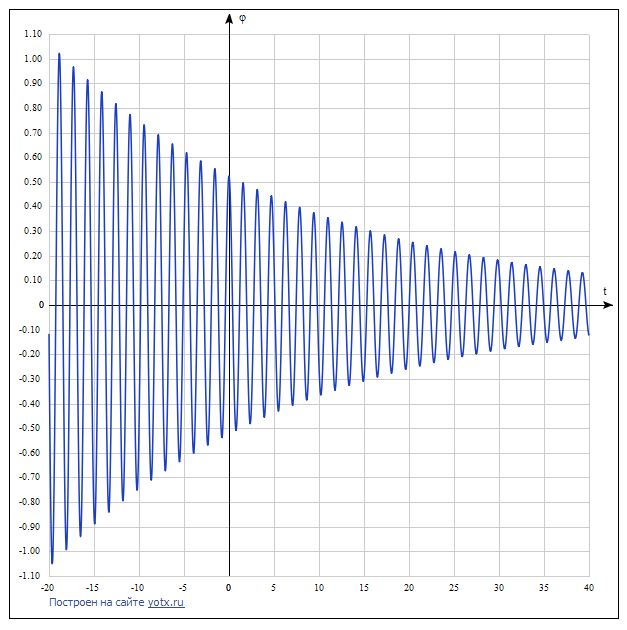
\includegraphics{yotx.ru (4).png}}
	\caption{$\varphi(t) = A_0e^{-\frac{t}{\tau}}\cos \omega t$}
	\label{framework1} %framework,fig1
\end{figure}

\begin{figure}[h]%current location
	\centering
	\scalebox{0.8}{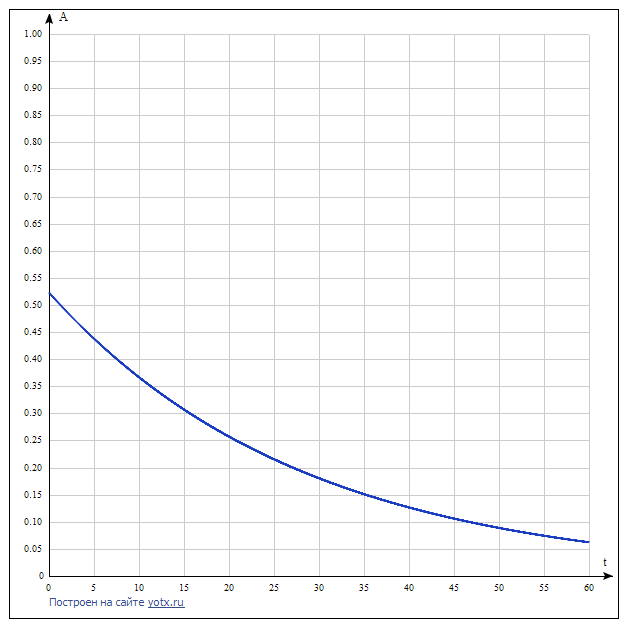
\includegraphics{yotx.ru (5).png}}
	\caption{$A(t) = A_0e^{-\frac{t}{\tau}}$}
	\label{framework2} %framework,fig1
\end{figure}

\newpage
\newpage

\section*{Вывод}

В ходе выполнения лабораторной работы были произведены исследования динамика колебательного движения на примере крутильного маятника. 
Были получены значения, основываясь на которых, были рассчитаны периоды колебаний маятника, 
время затухания маятника, собственные частоты его колебаний, коэффициент кручения, 
модуль сдвига материала подвеса, полная энергия, мощность потерь, модуль Юнга и добротность маятника. 
Исходя из полученных значений, можно сделать вывод, что значения, полученные экспериментально достаточно точны, то есть, эксперимент можно считать успешным.


\newpage

\end{document} 